%!TEX root = ../template.tex
%%%%%%%%%%%%%%%%%%%%%%%%%%%%%%%%%%%%%%%%%%%%%%%%%%%%%%%%%%%%%%%%%%%
%% chapter1.tex
%% NOVA thesis document file
%%
%% Chapter with introduction
%%%%%%%%%%%%%%%%%%%%%%%%%%%%%%%%%%%%%%%%%%%%%%%%%%%%%%%%%%%%%%%%%%%
\typeout{NT FILE chapter4.tex}%

\chapter{Methodology}
\label{chap:methodology}

In this chapter, we present the methodology and design approaches adopted for the development of the tool, explaining why they were appropriate for our project. First, we describe the project iterations that guided the implementation process and show how the system evolved step by step. Then, in the design, we present the approach, outlining the main stages followed during the design cycle.

\section{Model}
In software development, a model is a representation of a system that serves as a blueprint for its construction. Models help developers and stakeholders understand complex systems, explore solutions, and test designs before implementation. Just like architectural blueprints or small-scale 3D models, software models allow us to anticipate potential problems and make better decisions without committing resources too early [Model-Driven Software Development]. 

Models play a central role in software development. They help to improve understanding of both the problem and the solution and guide critical decisions during the project. High-quality models make the development process easier and increase the chances of producing a successful software system.

Software development can follow different models, each guiding how the system is planned, designed, and built. One well-known approach is the Waterfall model, which follows a linear and sequential process: requirements are collected first, followed by design, implementation, testing, and maintenance [https://dl.acm.org/doi/pdf/10.5555/41765.41801]. This model is simple and easy to manage, but it can be rigid when changes are needed. Agile organizes work in short cycles, emphasizes continuous feedback, and allows developers to respond quickly to changing requirements. These models provide frameworks that help developers structure the project, make decisions, and deliver reliable software efficiently [A Literature Review on Agile Model Methodology in software Development].

\subsection{Iterative Model}
The Iterative Model is a software development approach in which the system is built through repeated cycles, called iterations. Each iteration produces a version of the system that is more complete than the previous one, allowing the developer to refine the product gradually and respond to changes. This approach is useful for complex projects where requirements may evolve or where early feedback is important [Sommerville, I. (2016). Software Engineering (10th edition). Pearson]. The iterative model is basically divided into three key steps in each iteration:

\begin{itemize}
    \item \textbf{Design:} In this step, the solution for the iteration is planned, including the system architecture, interfaces, and data structures. It defines what will be built in the current cycle.
    \item \textbf{Implementation:} The planned features and components are developed and integrated into the system. This step produces a working version of the system for this iteration.
    \item \textbf{Evaluation:} The implemented features are tested to ensure they work correctly and meet the requirements. Feedback is collected to identify improvements, which guide the next iteration.
\end{itemize}

From all the software development models, the one most suited for our project is the Iterative Model. Given the characteristics of our project, which is large and complex, the iterative model provides the best fit. By dividing development into iterations, we can build the system gradually and manage time more effectively if unexpected difficulties appear. For example, some tasks may take longer than expected or we may face challenges in implementing certain features. On the other hand, if an iteration is completed faster than planned, we can adapt by adding new features or extra iterations.

Our project is ambitious because developing an online interactive tool for practicing \gls{ND} problems is not a simple task. It involves many aspects such as understanding how \gls{ND} problems work, implementing exercises correctly, creating an online platform, and supporting different environments for students and teachers. The system must handle user sessions, authentication, and permissions, and it should ensure security and privacy of data. It must also be scalable to support many simultaneous users and allow future expansions. In addition, we need to provide interactive feedback, hints, and automatic validation of exercises, a progress tracking system, and possibly a way to generate new problems automatically. The tool should also have a clear and intuitive user interface, support multiple devices, and allow teachers to manage exercises, and grade exercises. All these aspects demonstrate that the project involves many complex elements that must work together seamlessly.

The iterative approach fits this context very well. We can begin by developing a basic version of the tool with only essential features. Then in each iteration, we can gradually add more complex functionalities until we reach the final version. Iterations also serve as checkpoints, providing a functional version at the end of each cycle. Even if an iteration does not cover all requirements initially established, we still have a usable version that can be tested, used in practice, and extended by future developers.

This approach is safer and more flexible than trying to implement everything at once, as in the Waterfall model. The Waterfall model reflects a “do it right the first time” mindset [A Pipelined Approach for Iterative Software
Process Model], which originates from optimism and the belief that failure can be avoided. In practice, if problems occur or features take longer than expected, the final system may not be fully functional at the end of development.

In contrast, the Iterative Model follows a “fail fast” approach [A Pipelined Approach for Iterative Software Process Model], which recognizes that problems are a natural part of development. By building the system in repeated cycles, functional increments are produced throughout the project. This allows early detection of errors, adaptation to changing requirements, and continuous improvement, reducing risk and increasing flexibility compared to the Waterfall approach.

The whole purpose of iterative development is to find the risks hidden in the design of the previous iterations, correct them sooner, and progress further. Its purpose is to discover pitfalls that otherwise could not have been foreseen, ensuring that the system evolves safely and efficiently with each cycle.

\subsection{Iterations}
\label{it:iterations}
Our project was divided into different iterations, and at the end of each one, we planned to have a functional application that could be used to practice \gls{ND}. As mentioned earlier, a better approach is to start small and focus on the minimal requirements needed to have a fully functional online tool. This guided the first iteration. In this initial cycle, we created a basic version of the tool that allowed users to practice exercises. At this stage, there was no authentication, security, or user sessions, as the focus was on building a working foundation.

For the second iteration, we aimed to improve the previous version by introducing a simple feedback system. This system guided students during exercises and offered different levels of help, helping them understand their mistakes and learn from them.

In the third iteration, we planned to take the feedback system to a higher level by providing more complex guidance for students who were unsure how to progress in proofs. This iteration was developed separately because creating an algorithm to generate \gls{ND} proofs is a challenging task. The separation also ensured flexibility: if we failed to find an effective way to improve the feedback, we could always revert to the previous iteration without losing a functional version of the tool.

These three iterations formed the core plan from the beginning of the project. However, we never discarded the possibility of adding additional iterations to cover the remaining requirements and further improve the tool. This iterative approach allowed us to progress incrementally, test each version, and ensure that the system remained functional and expandable at every stage.

\begin{enumerate}
\setlength{\itemsep}{5pt}
    \item \textbf{First Iteration} \\
    \textbf{Goal:} Provide a functional platform for practicing \gls{ND} exercises. \\
    \textbf{Planned Features:}
    \begin{itemize}
        \item Simple and intuitive interface for practicing exercises
        \item Basic exercise management where students can select the exercises they want to practice
        \item A way to submit exercises for validation (without feedback)
    \end{itemize}

    \item \textbf{Second Iteration} \\
    \textbf{Goal:} Introduce a feedback system to guide students. \\
    \textbf{Planned Features:}
    \begin{itemize}
        \item Simple feedback for exercises based on semantic errors
        \item Multiple levels of feedback gradually increasing the detail of the reported errors to help students understand mistakes
        \item Improved interface from the first iteration, considering support for more devices such as touch screens
    \end{itemize}

    \item \textbf{Third Iteration} \\
    \textbf{Goal:} Provide advanced feedback and support for complex guidance. \\
    \textbf{Planned Features:}
    \begin{itemize}
        \item Algorithm to generate \gls{ND} proofs automatically for producing feedback
        \item More complex guidance for students stuck in proofs using the algorithm
        \item Improved interface based on the second iteration, enhancing the interactivity of the system
    \end{itemize}
\end{enumerate}

\section{User-Centered Design}
\gls{UCD} is both a design methodology and a philosophy that places the needs, goals, and success of the end user at the center of the development process [https://doi.org/10.1002/9781118786352.WBIEG0432]. The main idea is that systems should be designed not only to function correctly, but also to support real user tasks, be easy to operate, and provide clear value to the people who use them.

Although \gls{UCD} can be applied to any product or system intended for human use, it is most often associated with computer systems and software design. In this context, the success of the design is measured by how easily users can understand the system, how efficiently they can complete their tasks, and how satisfied they are with their overall experience.

One of the main characteristics of \gls{UCD} is that it usually reduces the need for heavy documentation or extensive training. Because the system is shaped around user expectations and abilities, it becomes more intuitive and easier to adopt. \gls{UCD} is not limited to interface design: it can also influence other parts of the system such as documentation and the way data is entered and presented.

The \gls{UCD} design is structured around stages that ensure user needs guide the development process [https://dx.doi.org/10.4324/9780203880869.ch49]. The first stage is User Analysis, which focuses on understanding who the users are, their characteristics, goals, and context of use. Once this understanding is established, the process moves to Task Analysis, where the tasks that users must perform with the system are examined. By breaking these tasks into smaller steps and studying how users approach them, the design can be shaped to support their activities more effectively and minimize errors. Finally, the stage of Requirements Analysis defines the functional and non-functional requirements based on the insights from the previous stages, ensuring that the system aligns with user needs while remaining technically feasible.

\gls{UCD} was chosen because the project focuses on students and teachers using an online tool for practicing \gls{ND} exercises. The design is guided by the needs, goals, and abilities of the users to ensure the tool is easy to use and understand. Interactivity is an important factor, so the design also focuses on creating engaging exercises and responsive feedback. By involving users during the design process, the tool can be refined iteratively to better support learning and provide a satisfying experience.

\subsection{User Analysis}
\label{user-analysis}
The first step of this design is to identify the target users who will interact with the system. We identified four main types of users:

\begin{itemize}
\setlength{\itemsep}{5pt}
    \item \textbf{Beginner Student:} A student who is just starting to learn \gls{ND} proofs and has little prior experience with exercises in this area. This type of user mainly seeks simple exercises that help them gain confidence and become familiar with the basic rules.
    \item \textbf{Intermediate Student:} A student who has some knowledge of \gls{ND} proofs and some practice solving exercises, familiar with basic steps and common strategies. Their main goal is to improve efficiency and accuracy while solving increasingly complex problems.
    \item \textbf{Experienced Student:} A student with advanced knowledge of \gls{ND} proofs, comfortable handling complex exercises and understanding detailed logical structures. This group is motivated by the challenge of solving demanding exercises that allow them to refine their skills further.
    \item \textbf{Teacher:} A user with strong expertise in \gls{ND} proofs, responsible for creating and testing exercises, guiding students during practice, and monitoring their learning progress.
\end{itemize}

Each of these user groups faces specific challenges. Students often struggle with identifying whether their reasoning is correct and understanding where they made mistakes, while teachers face difficulties in providing timely and personalized feedback to large groups. This tool aims to address both sides: giving students clearer guidance during practice and offering teachers resources to better support and track their learners.  

The context of use is also diverse. Students may use the tool at home, on tablets or computers, to practice individually, or during class for guided activities. Teachers, on the other hand, may use it while preparing teaching materials, assigning exercises, or evaluating student work.  

For all users, we assume familiarity with basic technologies, especially web platforms, so they understand how to navigate and interact with online tools. The distinction between three levels of students highlights that the application is designed to support different learning stages: from beginners just starting with \gls{ND}, to intermediates consolidating their knowledge, and advanced students seeking greater challenges. Teachers are considered separately because their role goes beyond solving exercises. They are also responsible for designing tasks, guiding learners, and overseeing progress. In addition, some teachers handle multiple subjects and may not teach \gls{ND} in every semester. When they return to this topic after a break, it can be challenging to remember the steps for constructing proofs. The tool can serve as a reference to quickly remind them how proofs are built and support their teaching.


\subsection{Task Analysis}
To determine which functionalities our tool should support, we needed to understand how users approach these exercises. There are several ways to perform a task analysis. One is observation, where we watch a student solve exercises step by step, although this can sometimes capture inefficient habits. Another approach is Expert Advice, where teachers explain how tasks should ideally be performed, which may differ from actual practice.

For this project, we used a combination of these methods. We observed a teacher solving exercises according to their teaching approach and incorporated expert advice from teachers. In addition, we drew on personal experience and consulted textbooks describing standard methods for solving \gls{ND} exercises. This mixed approach allowed us to capture both the practical challenges students face and the ideal strategies recommended by experts, providing a solid foundation for designing the tool’s features.

Since the iterations presented in \autoref{it:iterations} focus on a basic version of the system that only supports practicing exercises, our task analysis was limited to the process of constructing \gls{ND} proofs.

From our task analysis, we learned that there is no single way to start a proof. Some users begin from the conclusion, while others start from the premises and assumptions. The notation for rules follows a consistent structure: conclusions and hypotheses are separated by a horizontal line, with rule information on the right. Marks assigned to expressions are placed above them, following the notation presented in the rules [REF RULES]. As proofs progress, some students write assumptions on the side of the proof along with the mark numbers to keep track of them. In some \gls{FOL} rules, users note which variables must not appear free in open hypotheses. \autoref{fig:task-proof} shows an example of a completed tree proof created by a student, with assumptions listed on the right.

\begin{figure}[h]
\centering
\includegraphics[width=0.7\linewidth]{Chapters/Figures/task-proof.png}
\caption{Example of a final tree proof created by a student}
\label{fig:task-proof}
\end{figure}

During our observations, we identified several common challenges. Limited space on paper often forces students to erase and rewrite sections mid-proof. Students who do not record assumptions clearly spend extra time determining which assumptions can be applied at each step. Furthermore, many students are uncertain whether their reasoning is correct, leading to frustration and getting stuck on particular steps. These findings highlight the need for tool features that support flexible proof construction, guide learners, and provide feedback so that students can continue practicing efficiently.


\subsection{Requirements}
The next step in the \gls{UCD} approach is to extract functional and non-functional requirements based on the user and task analysis previously performed. In this section, we focus on the requirements for students, as the planned iterations only cover the construction of proofs and do not include features specifically for teachers.

\subsubsection*{User Requirements}
\begin{enumerate}
    \item Provide an online and interactive environment where students can practice \gls{ND} exercises.
    \item Allow students to practice exercises in tree format, covering both \gls{PL} and \gls{FOL}.
    \item Enable students to build proofs freely, similar to paper-based construction, without enforcing a strict sequence.
    \item Allow students to create multiple proofs for the same exercise and explore alternative strategies.
    \item Display the assumptions made at any point in the proof.
    \item Equip exercises with an advanced feedback and hint system:
    \begin{itemize}
        \item Report structural and conceptual errors.
        \item Provide different levels of guidance, from general hints to precise help.
        \item Automatically adapt the level of assistance based on the student's proficiency, inferred from past mistakes.
    \end{itemize}
    \item Allow students to check the solution of exercises.
    \item Provide access to solutions after submission to support self-study.
\end{enumerate}

\subsubsection*{Non-Functional Requirements}
\begin{enumerate}
    \item Support at least 60 simultaneous students, with response times under 100 ms for interactions.
    \item Be extensible to allow the integration of additional types of logic exercises in the future.
    \item Be compatible with multiple platforms, including desktops, tablets, and major web browsers.
\end{enumerate}

Students need an online and interactive environment because doing proofs on paper can make it hard to construct them, follow their reasoning, and keep track of assumptions. Using a tree format follows the standard way proofs are shown in classes and textbooks, which helps students apply what they have learned.

Allowing students to build proofs freely and try different strategies gives them room to experiment and explore. Showing assumptions at any point makes it easier to know which ones are active. The feedback and hints help students when they get stuck and adjust to their level of knowledge, reducing frustration and supporting learning.

Access to solutions and the ability to check exercises encourage self-study and reflection. Non-functional requirements like performance, compatibility, and the ability to add more features in the future make sure the tool works fast, can be used on different devices, and can grow without problems.

\subsection{Design}
Another important step in the \gls{UCD} process is the design phase. In this section, we present the evolution of our interface through the development of multiple prototypes, highlighting the design decisions, improvements, and changes made at each stage.

From the very beginning of development, our main concern was how to replicate on the computer the same steps a student would normally take to create a proof on paper. Designing a system where proofs and sub-proofs could be connected and expanded as new rules were applied was not a straightforward task, either conceptually or technically. As we also wanted touchscreens to support our application, we had to ensure that all interactions, could be performed easily through simple gestures. This requirement influenced many of our design decisions, since the interface needed to remain intuitive and responsive while still representing the logical structure of the proofs in a precise way.

One of the recurring problems when constructing proofs on paper is the limited space available. A typical example occurs when starting a proof from the top where multiple sub-proofs may be derived from the premises, and although they might eventually connect to other parts of the proof, if they are not written in the correct order, the whole structure has to be erased and redone. These challenges of rigid and insufficient space were key concerns that we wanted to address in our implementation.

In past projects that tried to implement this type of exercise, a common limitation was that proofs could only be built from the bottom, following a fixed order of reasoning. This was very different from working on paper, where students can explore different paths more freely. This was another major concern that we had in the design of our prototypes.

Our first idea was inspired by Lego pieces. We can think of a proof as a Lego piece that can be connected and disconnected from others, allowing us to simulate the construction of proofs. In the same way that Lego pieces can be put together from the bottom up or from the top down to form blocks, which can then be combined into bigger structures, proofs can also be built in a modular and flexible way.

\subsubsection{First Prototype}
Based on the Lego idea, we searched online for tools that would allow us to replicate the same concept. We found Google Blockly [REF], a visual programming library based on blocks, very similar to Scratch [REF]. In Blockly, programming instructions are represented as blocks that can be connected to create programs, as shown in \autoref{fig:google_blockly}. Using Blockly, we were able to define our own custom blocks and convert them into programs with actual lines of code. For example, we could create blocks for the application of rules, formulas, and marks and then convert into our custom language to represent proofs. However, a major concern arose early when we simulated the creation of proofs. The way blocks are connected does not exactly represent how proofs are constructed. Blockly follows a linearized structure where one block can only be placed below another. In contrast, our proofs follow a tree-shaped style which has a different structure. This becomes clear when we try to map a rule that requires multiple hypotheses, such as $\vee_E$ rule, which needs three hypotheses. With Blockly's structure, this is not possible because we cannot define three operations to run simultaneously and independently from each other.

\begin{figure}[h]
    \centering
    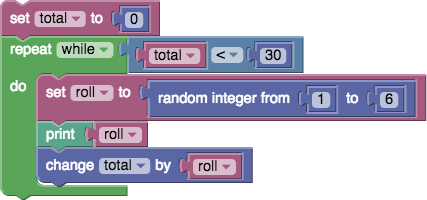
\includegraphics[width=0.6\linewidth]{Chapters/Figures/image6.png}
    \caption{Google Blockly example}
    \label{fig:google_blockly}
\end{figure}

From this first prototype we took many good ideas. For example, the idea of having our components represented as blocks that can be moved around and connected to each other depending on the type of block. The Blockly environment provides a sidebar where users can drag blocks into the construction area. In this area, we can place multiple blocks, some attached and others not. We can also delete and duplicate blocks. With these features in mind, we created our next prototype.

\subsubsection{Second Prototype}
Our biggest concern in this prototype was related to the orientation in which proofs are constructed. As previously mentioned, we wanted to keep the construction of proofs as close as possible to the way we do it on paper. Therefore, we came up with the idea that instead of connecting blocks sequentially, one after another, we would nest blocks vertically by placing blocks inside others. This approach allows us to simulate the construction of proofs more accurately. With this idea, we developed the second prototype, shown in \autoref{fig:it-2.1}. In this version, users could drag predefined blocks from the sidebar into the building environment, and these blocks could then be placed inside other blocks to form larger structures. As illustrated in \autoref{fig:it-2.1}, the largest block displays different shades of gray that represent the nested sub-blocks. At this stage, we had not yet planned how formulas, marks, and rules would be inserted.

We aimed to keep the interface very simple and as intuitive as possible, so that new users could understand how it works without the need for a tutorial. For example, the previews of the rules displayed both in the sidebar and in the building environment followed a structure very similar to the rules presented in [REF RULES].


\begin{figure}[h]
    \centering
    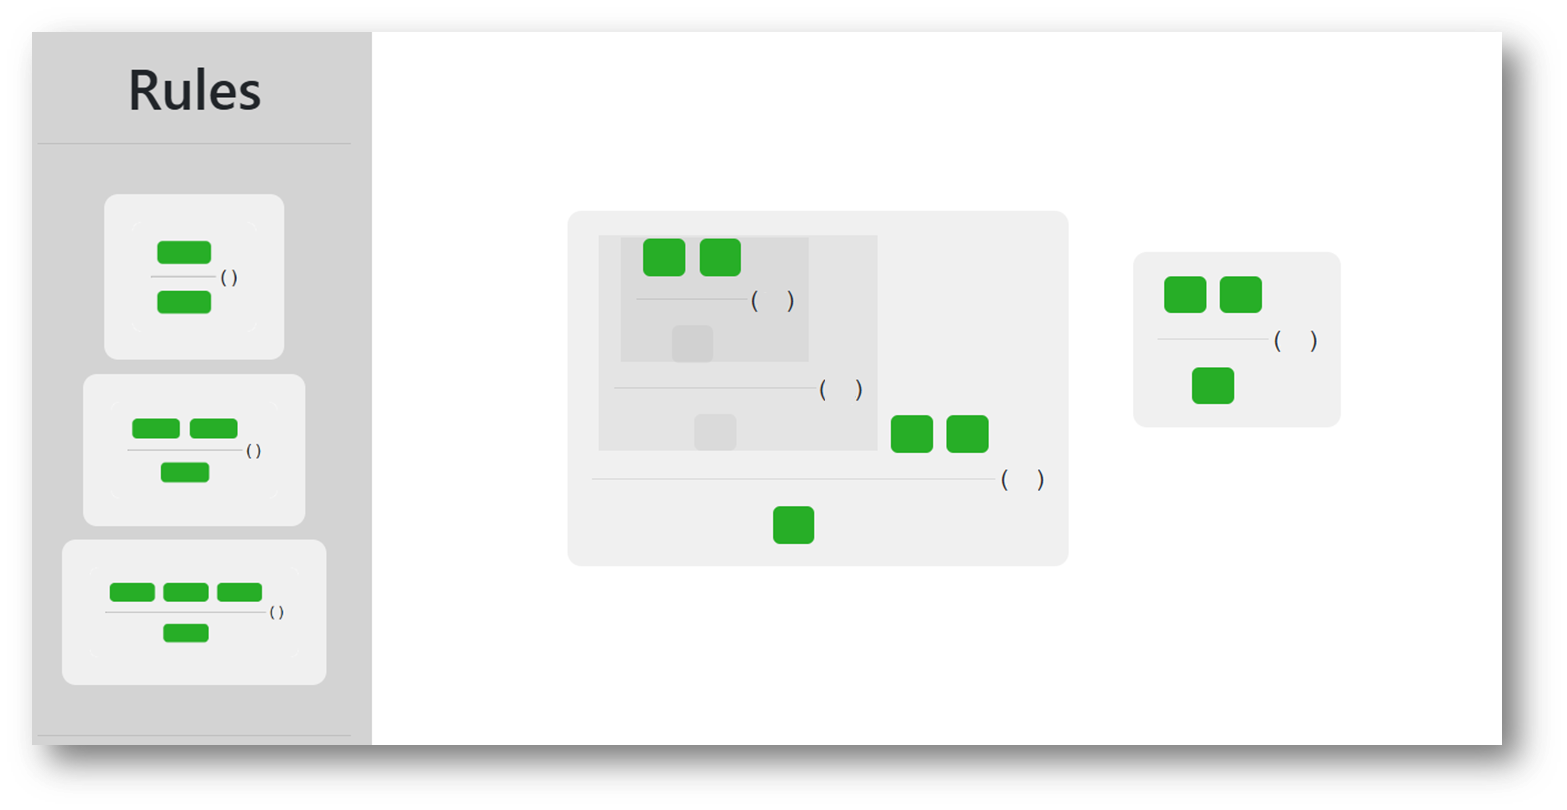
\includegraphics[width=0.95\linewidth]{Chapters/Figures/image3.png}
    \caption{Graphical interface of the proof-building environment in the second prototype.}
    \label{fig:it-2.1}
\end{figure}

However, we had plans for how to display information about the proof being constructed. As shown in \autoref{fig:it-2.1}, users could view the current state of the proof by selecting a formula. In this example, by selecting the formula $\psi \land \gamma$ (highlighted in yellow), the system displays information about the part of the problem that remains unsolved, as well as the list of hypotheses that were generated at that point in the proof. This feature is very useful, as it helps users recall the assumptions that were previously made. In handwritten proofs, these assumptions are usually written on the right side of the proof to remind us of what has been assumed.

\begin{figure}[h]
    \centering
    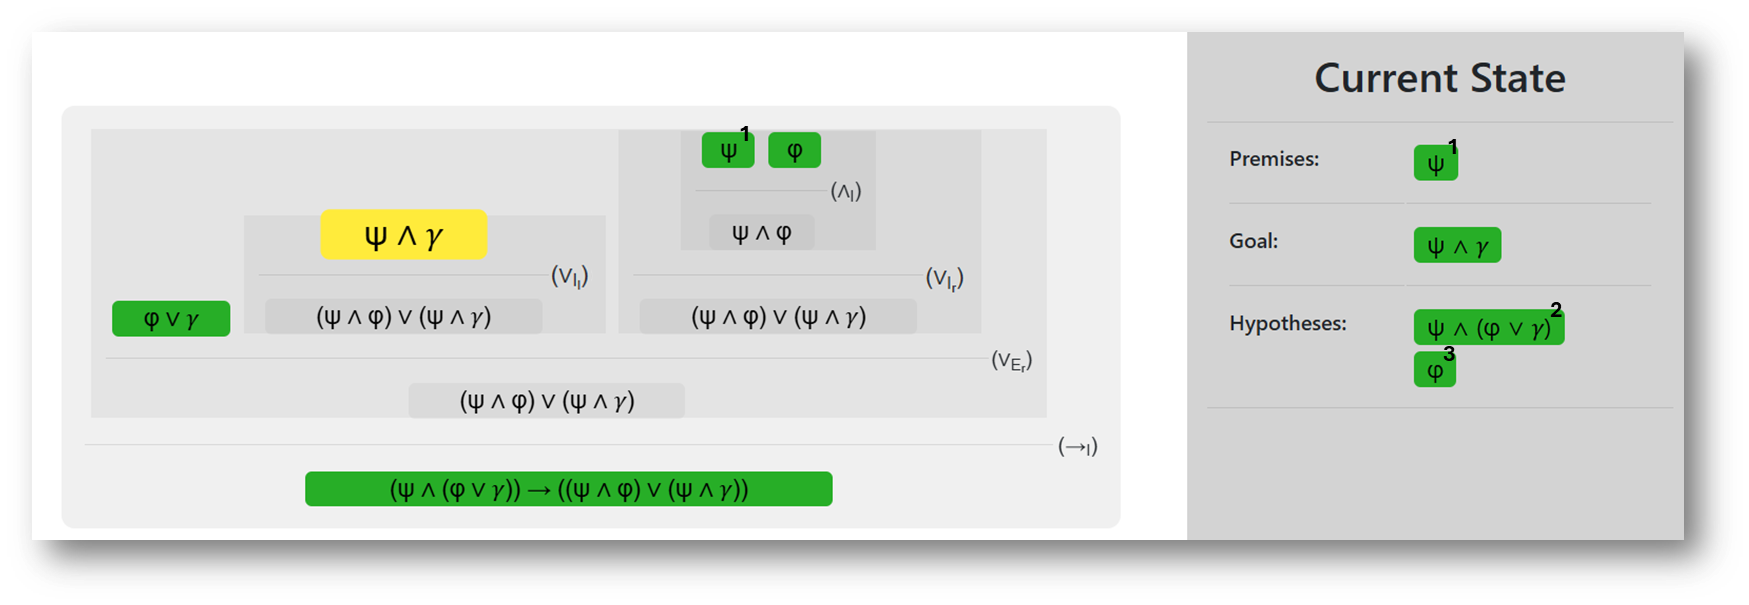
\includegraphics[width=0.95\linewidth]{Chapters/Figures/image4.png}
    \caption{Graphical interface of the proof-building environment showing the current state of the proof in the second prototype.}
    \label{fig:it-2.2}
\end{figure}

Another topic that we also took into consideration was how errors and feedback would be displayed in the proofs. At this stage, we planned to highlight entire parts of the proof with a different color scheme, depending on whether it was an error, a warning, or feedback. The message assigned to the error would then appear at the bottom of the page. However, we ended up abandoning this idea because it was not viable in cases where the building environment contained multiple proofs or when the error messages were too long to be fully displayed on the screen. \autoref{fig:it-2.2} shows how the highlights and messages would appear on the screen.

\begin{figure}[h]
    \centering
    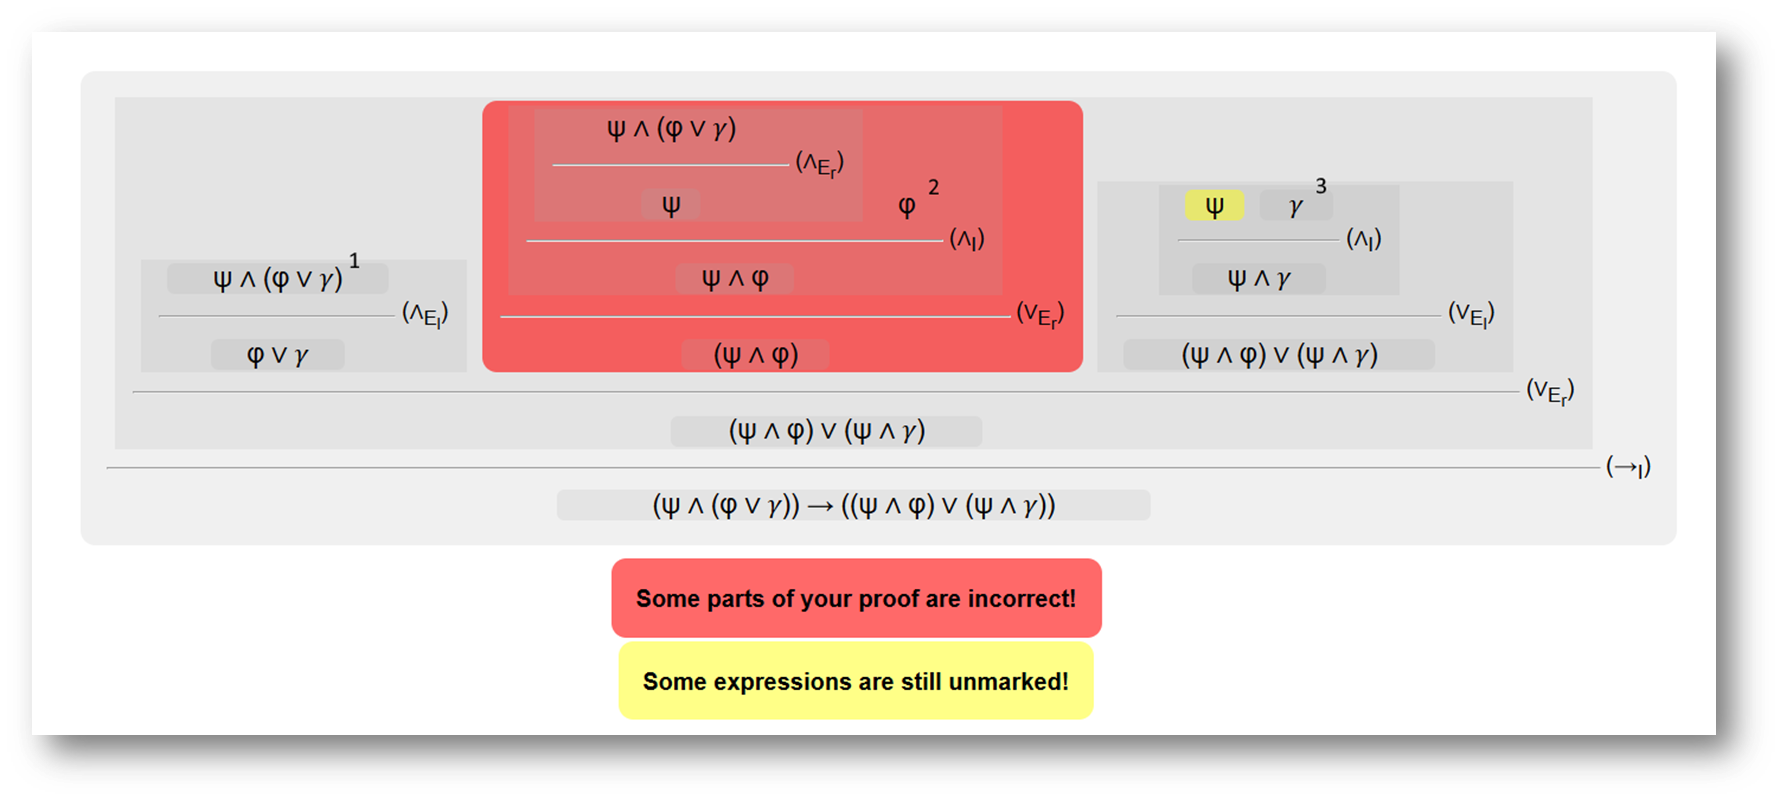
\includegraphics[width=0.95\linewidth]{Chapters/Figures/image5.png}
    \caption{Graphical interface of the proof-building environment showing highlights and messages for a proof in the second prototype.}
    \label{fig:it-2.3}
\end{figure}

By the end of this prototype, we had not yet defined how formulas, rules, and marks would be inserted into the blocks. Addressing this issue became the main focus of the next prototype.

\subsubsection{Third Prototype}

In this prototype, we explored several ways in which blocks could be filled with information. We initially considered using input boxes for formulas and dropdown menus to select marks and rules. However, we adopted a different approach. In this prototype, we created blocks for every element, not only for rule application but also for formulas, rule names, and marks. The idea was that when a user dragged one of these components from the sidebar into the building environment, a prompt would appear asking the user to insert a value, depending on the type of block, and then the component would be added to the environment. Each component had a different shape: formulas were shown as rounded rectangles, marks as circles, rule names as rectangles, and dashed boxes represented empty places waiting for a component, as illustrated in \autoref{fig:it-3.1}.

\begin{figure}[h]
    \centering
    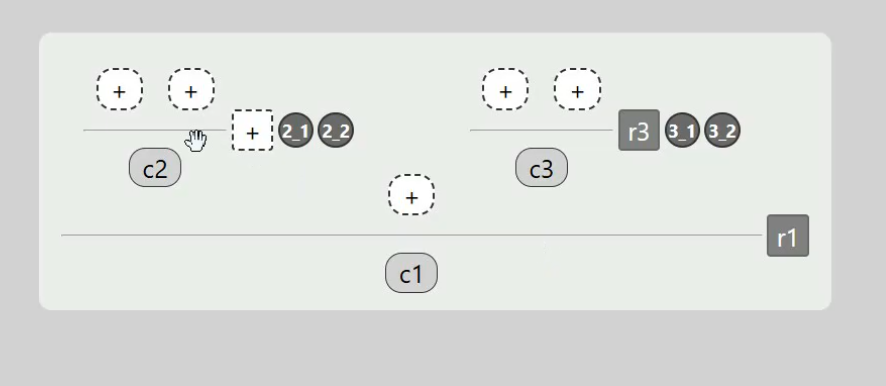
\includegraphics[width=0.72\linewidth]{Chapters/Figures/image1.png}
    \caption{Graphical interface of the proof components in the third prototype.}
    \label{fig:it-3.1}
\end{figure}

To construct even a small proof, the user had to add every individual formula either by dragging it or by clicking the plus button in the proofs to fill the proof. This design choice proved to be inefficient, as constructing proofs took significantly more time.

In addition, we added an auxiliary keyboard to the interface to help users insert logical symbols, since conventional keyboards do not have these symbols. The keyboard would appear whenever a user double-clicked on a formula or when a new formula was added to the environment. \autoref{fig:it-3.2} shows an example of a formula being edited.

\begin{figure}[h]
    \centering
    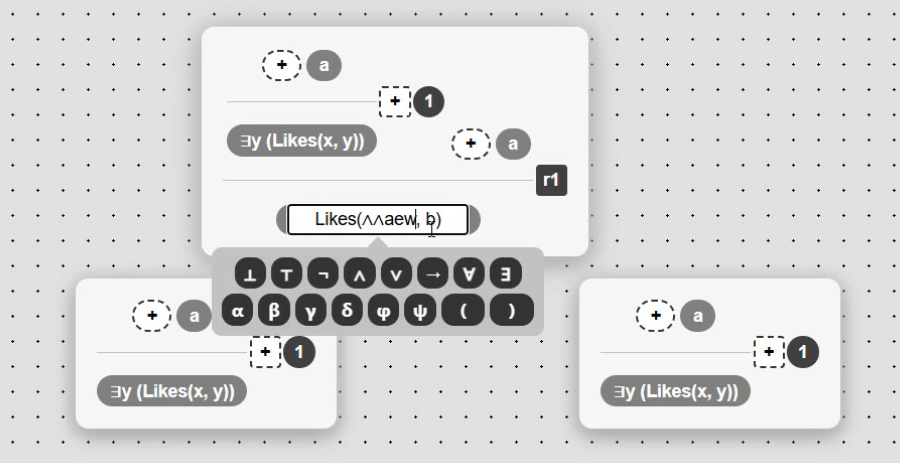
\includegraphics[width=0.95\linewidth]{Chapters/Figures/image2.png}
    \caption{Graphical interface of the auxiliary keyboard for inserting and editing formulas in the third prototype.}
    \label{fig:it-3.2}
\end{figure}

Some other quality-of-life features were also considered in this prototype, such as the option to delete a proof by dragging the whole proof to a trash bin, the ability to undo and redo operations in the environment, the addition of a dotted background to provide spatial guidance and alignment of the proofs, as well as animations when components were dragged and dropped, among many other features.

The final design, addressed the issue where users previously had to drag every single element to build proofs. In the final version, a proof is treated as a single component, and its internal elements can be edited by clicking on them. For marks, the previous auxiliary keyboard is shown, while for formulas and rule names a dropdown menu appears. Section~\ref{sec:final-interface} describes the complete workflow of the final interface and explains how users interact with the application.

\subsection{Evaluation}
Evaluation is an important part of the \gls{UCD} process, as it allows us to check if the system supports the needs and tasks identified earlier. In our case, the goal was to assess whether the interface was usable, interactive, and provided meaningful feedback during proof construction.

To do this, we organized online meetings with different types of users (beginner, intermediate, and experienced students, as well as teachers). During these sessions, participants were asked to complete a series of exercises using the system. The evaluation focused on three main aspects:

\begin{itemize}
    \item \textbf{Usability of the interface:} We assessed whether the interface was clear, easy to understand, and whether users could efficiently complete exercises without unnecessary effort.
    \item \textbf{Interactivity of proof construction:} We examined how well the system supported natural interaction when building proofs, such as adding marks, rules, nesting and unnesting sub-proofs. These interactions were tested on both desktop and touchscreen devices to ensure consistency.
    \item \textbf{Effectiveness of the feedback system:} We evaluated whether the feedback helped users identify mistakes, understand why errors occurred, and receive useful hints without disrupting the proof-building process.
\end{itemize}

After completing the tasks, participants were asked to fill in a \gls{SUS} questionnaire, a simple and widely used tool that measures how easy and satisfying a system is to use [REF https://doi.org/10.1080/10447318.2018.1455307]. The detailed analysis of the evaluation results is presented in [REF-RESULTS].

